\chapter{Úvod}
\label{uvod}
%úvod práce
%úvod do problému
%popis struktury práce


\chapter{Hudební teorie}
% základy hudební nauky
Nejen pro harmonizaci melodie je potřeba znát hudební nauku. 
V této kapitole budou nastíněny základy a pojmy hudební nauky, 
tedy co to jsou tóny, noty, jejich vlastnosti a stupnice. 
Dále bude rozdělena melodie a harmonie a popsány akordy a tóniny. \par 

\section*{Tóny}
Chvěním těles, které rozechvívají okolní vzduch, vzniká zvuk, 
tedy to co slyšíme. 
Nepravidelným chvěním vznikají hluky. 
Naopak zvuky vznikající pravidelným kmitáním tělesa nazýváme tóny. 
V hudbě jsou především využívány právě tóny. 
Ty mají čtyři základní vlastnosti. \par

Podle různé doby chvění pružného tělesa rozlišujeme délku tónu. 
Další vlastností je síla, která je dána vzdáleností krajních bodů,
mezi nimiž těleso kmitá.
Tato vzdálenost se také označuje rozkmit nebo amplituda.
Velikost amplitudy je přímo úměrná síle, hlasitosti tónu.
Podle původu rozlišujeme barvu, někdy také témbr tónu.
Barva závisí na počtu znějících alikvotních tónů,
které se rozezní současně s hlavním hraným tónem. 
To je závislé na materiálu chvějícího se tělesa.
Pro představu, lze rozeznat, zda zní klavír, housle, trumpeta, či mužský nebo ženský hlas, 
navzdory tomu, že všechny mají stejnou výšku. 
Rozmanitou barvitost mají především velké orchestry.
Výšku tónu určujeme podle frekvence chvění, čili počtu kmitů za vteřinu. 
Čím vyšší frekvence, tím vyšší tón, a čím nižší frekvence, tím hlubší tón.\cite{zenkl,cmiral} \par

\section*{Soustava a jména tónů}
Tónová soustava je přehledné uspořádání všech tónů užívaných v hudbě.
Z vlastností tónů, vyjmenovaných výše, tónová soustava bere v úvahu pouze výšky tónu. 
Současnou tónovou soustavu tvoří sedm základních tónů, které
byly v minulosti označeny písmeny obyčejné abecedy: a, b, c, d, e, f, g.
Později se jako počátek hudební abecedy určilo písmeno c 
a písmeno b se nahradilo písmenem h.
Tím vzniká nynější hudební abeceda c, d, e, f, g, a, h.\par
Těchto sedm tónů se pravidelně opakují ve vyšších a nižších polohách.
Při postupu od výchozího c k nejbližšímu následujícímu, respektive předchozímu, c nacházíme osm stupňů 
(včetně obou c).
Vzdálenost mezi dvěma tóny stejného jména se proto nazývá oktáva (z latinského octo - osm).
Tónová soustava má oktáv devět.
Jelikož se základní tóny opakují stejnými jmény v různé výši,
jsou tyto oktávy dále pojmenovány.
Díky tomu má každý jednotlivý tón nejen svůj vlastní název,
ale také ustálené označení (viz tabulka \ref{tabulkaOktav}).
Například tón e v dvoučárkové oktávě se nazývá dvoučárkové e
a značí se buď $e^2$, nebo{ e''}.\cite{zenkl,cmiral}\par

\begin{table}[]
    \begin{tabular}{ l l l l l l l | l }
        $C_2$ & $D_2$ & $E_2$ & $F_2$ & $G_2$ & $A_2$ & $H_2$ & Subkontra oktáva    \\
        $C_1$ & $D_1$ & $E_1$ & $F_1$ & $G_1$ & $A_1$ & $H_1$ & Kontra oktáva       \\
        C     & D     & E     & F     & G     & A     & H     & Velká oktáva        \\
        c     & d     & e     & f     & g     & a     & h     & Malá oktáva         \\
        $c^1$ & $d^1$ & $e^1$ & $f^1$ & $g^1$ & $a^1$ & $h^1$ & Jednočárková oktáva \\
        $c^2$ & $d^2$ & $e^2$ & $f^2$ & $g^2$ & $a^2$ & $h^2$ & Dvoučárková oktáva  \\
        $c^3$ & $d^3$ & $e^3$ & $f^3$ & $g^3$ & $a^3$ & $h^3$ & Tříčárková oktáva   \\
        $c^4$ & $d^4$ & $e^4$ & $f^4$ & $g^4$ & $a^4$ & $h^4$ & Čtyřčárková oktáva  \\
    \end{tabular}
    \caption{Značení tónů a názvy jednotlivých oktáv}
    \label{tabulkaOktav}
\end{table}

Kromě označení tónů písmeny se lze také setkat se solmizačními slabikami do, re, mi, fa, sol, la, si,
které v 10. století zavedl italský mnich Guido z Arezza\cite{cmiral}.\par    

\section*{Alterace}
Každý ze základních tónů tónové soustavy můžeme jednou nebo dvakrát snížit nebo zvýšit.
Takto zvýšené a snížené tóny se souhrnně nazývají odvozené nebo alternované.
Alterace je pak shrnující název pro zvyšování a snižování tónů.
Zvýšení tónu značíme příponou -is v jeho názvu.
Naopak snížení označujeme příponou -es.
Existují ovšem různé výjimky.
Například snížením tónů~e~a~a získáme es, respektive as.
Pro snížené h se, místo hes, používá název~b.\cite{zenkl}\par

Alterace posunuje tón vždy právě o půltón, 
což je nejmenší vzdálenost mezi dvěma tóny užívaná v naší hudbě.
Celý tón je pak tvořen dvěma půltóny. 
V rozmezí oktávy se nachází dva půltóny ({e-f, h-c}), a pět celých tónů.
Dohromady oktáva sestává z dvanácti půltónů.
Přehledné uspořádání tónů a půltónů v oktávě lze vidět na klaviaturách klávesových nástrojů (viz obrázek \ref{obrazekRozlozeniKlaviatury}).
Základní tóny leží na bílých klávesách, jejich alterace pak na černých.\cite{zenkl,cmiral}\par

Můžeme si všimnout tónů, které mají stejnou výšku, ale různá jména.
Těmto tónům říkáme enharmonické, enharmonická záměna je pak nahrazení tónu tónem stejné výšky, ale jiného jména.\cite{zenkl}

\begin{figure*}[ht]\centering
    \centering
    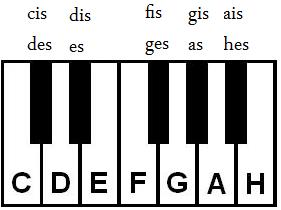
\includegraphics[width=0.4\linewidth]{obrazky/klaviatura.jpg}\\[1pt]  
    \caption{Přehledné uspořádání tónů a půltónů v oktávě \cite{orientaceNaKlaviature}}    
    \label{obrazekRozlozeniKlaviatury}
\end{figure*}

\section*{Noty}
%   noty (délky, výšky)
Alfabetické znaky nejsou pro značení tónů dostatečné, protože popisují pouze výšku tónu.
Pro hru na hudební nástroj, nebo skládání hudby je potřeba specifikovat také zbývající vlastnosti.
Po staletí trvajícím vývoji se ustálil a používá se notopis.
Základem jsou noty a notová osnova, kterou tvoří pět linek a čtyři mezery.
Noty se zapisují na linky i do mezer.
Takto lze zapsat pouze devět not.
Notovou osnovu však můžeme rozšířit pomocnými linkami nad, popřípadě pod notovou osnovou. 
Pomocné linky zapisujeme pouze tak dlouhé, jak je nezbytně nutné.
Pro snadnou orientaci v osnově se v praxi počítají linky a mezery směrem nahoru (s vyjímkou pomocných linek pod osnovou). 
Linky a mezery se počítají zvlášť. 
První mezera je mezi první a druhou linkou.\par

\label{ TODO Obrazek notove osnovy} 

Samotné noty jsou písemné značky pro tóny.
Tvar noty vyjadřuje délku noty a pozice v notové osnově její výšku.
Nota se skládá z několika částí.
Hlavička určuje pozici noty, a může být buď vyplněná , nebo nevyplněná . 
Nožka opět buď může být, a nebo nemusí . 
Pokud nota nožku má, pak ji, u not na třetí, prostřední lince a vyšších, píšeme směrem dolů ,
a naopak u nižších not směrem nahoru.
I toto pravidlo má ovšem nějaké výjimky.
Poslední částí noty je praporec, těch může mít nota nula až čtyři .
Pokud je za sebou víc not s praporci, lze je spojit, a praporce nahradit trámci.
V hudbě se používají tyto základní noty:

%\begin{itemize}
%    \item \wholeNote celá
%    \item \halfNote \halfNoteDown půlová
%    \item \quarterNote \quarterNoteDown čtvrťová
%    \item \eighthNote \eighthNoteDown osminová
%    \item \sixteenthNote \sixteenthNote šestnáctinová
%    \item \thirtysecondNote \thirtysecondNoteDown dvaatřicetinová
%\end{itemize}

Podle názvů not je zřejmé, že nota celá má délku dvou půlových not, čtyř čtvrtinových osmi osminových a tak dále.
Nejbližší nižší nota má délku poloviční a nejbližší vyšší dvojnásobnou.\par

Jména (výšky) not v osnově jsou určeny takzvaným klíčem, který se píše vždy na začátek každého řádku.
Klíčem se označuje pozici a jméno jedné notě a od ní se pojmenují ostatní v pořadí.
Pojmenování se řídí hudební abecedou.

% akordy (?)
% melodie / harmonie
% tóniny a stupně

\chapter{Reprezentace dat}
% ABC, MIDI, GUIDO ... viz NOTES.md


\chapter{Přehled přístupů automatické harmonizace}
% viz 04_Automatic Melody Harmonization with Triad Chords - A Comparative Study.pdf


\chapter{Strojové učení}
% rešerše strojového učení, jak funguje
% neuronové sítě
% frameworky ... viz NOTES.md

\chapter{Návrh systému}
% popis systému, který bude výstupem práce
% vstupy
% způsob práce
% výstup

\chapter{Implementace}
% popis implementace

\chapter{Experimenty}
% experimentování s implementovaným systémem
% představení výsledků

\chapter{Diskuse}
% diskuse výsledků
% jak je použít
% srovnání s cizími pracemi a papery

\chapter{Závěr}
\label{zaver}
% shrnutí práce
% možný budoucí vývoj práce
% celkový přínos
